%%%%%
%@TheDoctorRAB
%%%%%
%
%%%%%
%standard report format for journal papers
%%%%%
%
%%%%%
%PDF tagging accessible file
%compile with pdflatex
%run $show-pdf-tags --xml filename.pdf
%%%%%
%
%%%%%
%REFERENCES
%neup.bst - numbered citations in order of appearance, short author list with et al in reference section
%nsf.bst - numbered citations in order of appearance, full author list in references section
%standard.bst - citations with author last name with et al for more than 2 authors; full author list in references section
%ans.bst is for ANS only. 
%
%author = {Lastname, Firstname and Lastname, Firstname and Lastname, Firstname} for all bst formats
%bst renders the author list itself
%
%author = {{Nuclear Regulatory Commission}} if the author is an organization, institution, etc., and not people
%
%title = {{}} for all
%
%for all - use \citep{-} - [1] or (Borrelli, 2021) in the text
%standard.bst \cite{-} - Borrelli (2021) in the text
%standard.bst lists references alphabetically
%the rest list numerically
%%%%%


%%%%% enable tagging for accessibility
%\DocumentMetadata{
%    tagging=on,
%    check-tagging-status,
%    pdfversion=2.0,
%    pdfstandard=ua-2,
%    lang=en-US,
%    debug={log=all},
%    testphase={latest,tagpdf},
%    tagging-setup={math/setup={mathml-AF,mathml-SE}}
%}
%\tagpdfsetup{math/alt/use}

%%%%% general 
\documentclass[11pt,a4paper]{article}
\usepackage[lmargin=1in,rmargin=1in,tmargin=1in,bmargin=1in]{geometry}
\usepackage[pagewise]{lineno} %linenumbering restarts each page
%\usepackage[running]{lineno} %linenumbering continuous
\usepackage{mmap} %helps make pdfs copy and paste
\usepackage{setspace}
\usepackage{ulem} %strikethrough - do not \sout{\cite{}}
\usepackage[dvipsnames,table]{xcolor} %change font color (table loads colortbl)
\usepackage{graphicx}
\usepackage{tablefootnote}
\usepackage{footnotehyper}
\usepackage{float}
%\usepackage{mypythonhighlight,verbatim}
%\usepackage{subfig}
\usepackage[yyyymmdd]{datetime} %date format
\renewcommand{\dateseparator}{.}
%\graphicspath{{$TEXIMG/}} %path to graphics
\setcounter{secnumdepth}{5} %set subsection to nth level
\usepackage{needspace}
\usepackage[stable,hang,flushmargin]{footmisc} %footnotes in section titles and no indent; standard.bst
\usepackage[inline]{enumitem} %https://www.tug.org/texlive//Contents/live/texmf-dist/doc/latex-dev/latex-lab/latex-lab-enumitem.pdf
\usepackage{boldline}
\usepackage{makecell}
\usepackage{booktabs}
\usepackage{amssymb}
\usepackage{gensymb}
\usepackage{amsmath,nicefrac}
\usepackage{physics}
\usepackage{lscape}
\usepackage{array}
\usepackage{chngcntr}
\usepackage{sectsty}
\usepackage{textcomp}
\usepackage{lastpage}
\usepackage{xargs} %for \newcommandx
\usepackage[colorinlistoftodos,prependcaption,textsize=tiny]{todonotes} %makes colored boxes for commenting
\usepackage{soul}
\usepackage{color}
\usepackage{marginnote}
\usepackage[figure,table]{totalcount}
\usepackage{parskip}
\usepackage{listings} %allows python to be shown in text
\usepackage{xcolor}
%%%%%
\lstset{
  language=Python,
  basicstyle=\ttfamily\small,
  keywordstyle=\color{blue},
  commentstyle=\color{gray},
  stringstyle=\color{orange},
  numbers=left,
  numberstyle=\tiny,
  frame=single,
  breaklines=true,
  showstringspaces=false
}
%%%%%%%%%



%%%%% links and tags
\usepackage{hyperref}
\hypersetup{
    colorlinks,
    linkcolor=black,
    citecolor=black,
    urlcolor=blue,
    pdftitle={Homework},
    pdfauthor={R. A. Borrelli},
    pdfkeywords={homework},
    pdflanguage={en-US},
    pdfsubject={homework},
    pdfdisplaydoctitle=true 
} 
\usepackage[capitalise]{cleveref} %must be loaded after hyperref
%%%%%


%%%%% tikz
\usepackage{pgf}
\usepackage{tikz} % required for drawing custom shapes
\usetikzlibrary{shapes,arrows,automata,trees}
%%%%%


%%%%% fonts
\usepackage{times}
%arial - uncomment next two lines
%\usepackage{helvet}
%\renewcommand{\familydefault}{\sfdefault}
%%%%%


%%%%% references
%\usepackage[round,semicolon]{natbib} %for (Borrelli 2021; Clooney 2019) - standard.bst 
\usepackage[numbers,sort&compress]{natbib} %for [1-3] - nsf.bst, neup.bst
\setlength{\bibsep}{7pt} %sets space between references
\renewcommand{\bibsection}{\section*{\centering\bfseries\refname}} %bold, centered References heading
%\renewcommand{\bibsection}{} %suppresses large 'references' heading
%\renewcommand\bibpreamble{\vspace{\baselineskip}} %sets spacing after heading if not using default references heading
%%%%%


%%%%% tables and figures
\usepackage{longtable} %need to put label at top under caption then \\ - use spacing
\usepackage{tablefootnote}
\usepackage{tabularx}
\usepackage{multirow}
\usepackage{tabto} %general tabbed spacing
\usepackage{pdfpages}
\usepackage{wrapfig} %wraps figures around text
\setlength{\intextsep}{0.00mm}
\setlength{\columnsep}{1.00mm}
\usepackage[singlelinecheck=false,labelfont=bf]{caption}
\usepackage{subcaption}
\captionsetup[table]{justification=centering,skip=5pt,labelformat={default},labelsep=period,name={Table}} %sets a space after table caption
\captionsetup[figure]{justification=justified,skip=5pt,labelformat={default},labelsep=period,name={Figure}} %sets space above caption, 'figure' format
\captionsetup[wrapfigure]{justification=centering,aboveskip=0pt,belowskip=0pt,labelformat={default},labelsep=period,name={Fig.}} %sets space above caption, 'figure' format
\captionsetup[wraptable]{justification=centering,aboveskip=0pt,belowskip=0pt,labelformat={default},labelsep=period,name={Table}} %sets space above caption, 'figure' format
%%%%%


%%%%% watermark
%\usepackage[firstpage,vpos=0.63\paperheight]{draftwatermark}
%\SetWatermarkText{\shortstack{DRAFT\\do not distribute}}
%\SetWatermarkScale{0.20}
%%%%%


%%%%% cross referencing files
%\usepackage{xr} %for revisions - will cross reference from one file to here
%\externaldocument{/path/to/auxfilename} %aux file needed
%%%%%


%%%%% toc and glossaries
\usepackage[toc,title]{appendix}
\usepackage[acronym,nomain,nonumberlist]{glossaries}
\makenoidxglossaries
%do not load titlesec,titletoc
%%%%%


%%%%% editing
\newcommand{\edit}[1]{\textcolor{blue}{#1}} %shortcut for changing font color on revised text
\newcommand{\fn}[1]{\footnote{#1}} %shortcut for footnote tag
\newcommand*\sq{\mathbin{\vcenter{\hbox{\rule{.3ex}{.3ex}}}}} %makes a small square as a separator $\sq$
%\newcommand{\sk}[1]{\sout{#1}} %shortcut for default strikethrough - do not sk through citep
\newcommand\sk{\bgroup\markoverwith{\textcolor{red}{\rule[0.5ex]{1pt}{1pt}}}\ULon} %strikethrough with red line; not in \section{}
%\st{} does strikethrough using soul package but does not like acronyms
\newcommand{\blucell}{\cellcolor{aliceblue}} %use to shade in table cell
\newcommand{\grycekk}{\cellcolor{lightgray}} %use to shade in table cell
\newcommand{\whicell}{\cellcolor{antiquewhite}} %use to shade in table cell
%%%%%


%%%%% colors
%http://latexcolor.com/
%https://en.wikibooks.org/wiki/LaTeX/Colors#:~:text=black%2C%20blue%2C%20brown%2C%20cyan,be%20available%20on%20all%20systems.
\definecolor{aliceblue}{rgb}{0.94, 0.97, 1.0}
\definecolor{antiquewhite}{rgb}{0.98, 0.92, 0.84}
\definecolor{lightmauve}{rgb}{0.86, 0.82, 1.0}
\definecolor{brilliantlavender}{rgb}{0.96, 0.73, 1.0}
\definecolor{brandeisblue}{rgb}{0.0, 0.44, 1.0}
\definecolor{darkmidnightblue}{rgb}{0.0, 0.2, 0.4}

\newcommand{\x}{\cellcolor{aliceblue}} %use to shade in table cell
\newcommand{\y}{\cellcolor{lightgray}} %use to shade in table cell
\newcommand{\z}{\cellcolor{antiquewhite}} %use to shade in table cell
%%%%%


%%%%% acronyms
\newcommand{\acf}{\acrfull} %full acronym
\newcommand{\acl}{\acrlong} %long acronym
\newcommand{\acs}{\acrshort} %short acronym

\newcommand{\acfp}{\acrfullpl} %full acronym plural
\newcommand{\aclp}{\acrlongpl} %long acronym plural
\newcommand{\acsp}{\acrshortpl} %short acronym plural
%%%%%


%%%%% todonotes
\newcommandx{\cmt}[2][1=]{\todo[author=\textbf{STRUCTURE},tickmarkheight=0.15cm,linecolor=red,backgroundcolor=red!25,bordercolor=black,#1]{#2}}
\newcommandx{\con}[2][1=]{\todo[author=\textbf{CONTENT},tickmarkheight=0.15cm,linecolor=brilliantlavender,backgroundcolor=brilliantlavender,bordercolor=black,#1]{#2}}
\newcommandx{\rab}[2][1=]{\todo[noline,author=\textbf{RAB},backgroundcolor=Plum!25,bordercolor=black,#1]{#2}}


%\newcommandx{\jon}[2][1=]{\todo[noline,author=\textbf{ATTN: Johnson},backgroundcolor=blue!25,bordercolor=black,#1]{#2}}
%\newcommandx{\han}[2][1=]{\todo[noline,author=\textbf{ATTN: Haney},backgroundcolor=OliveGreen!25,bordercolor=black,#1]{#2}}
%\newcommandx{\rab}[2][1=]{\todo[author=\textbf{RAB},tickmarkheight=0.15cm,linecolor=Plum,backgroundcolor=Plum!25,bordercolor=black,#1]{#2}}
%\newcommandx{\han}[2][1=]{\todo[author=\textbf{ATTN: Haney},tickmarkheight=0.15cm,linecolor=OliveGreen,backgroundcolor=OliveGreen!25,bordercolor=OliveGreen,#1]{#2}}
%\newcommandx{\jon}[2][1=]{\todo[author=\textbf{ATTN: Johnson},tickmarkheight=0.15cm,linecolor=blue,backgroundcolor=blue!25,bordercolor=blue,#1]{#2}}


% highlighting 
\DeclareRobustCommand{\hlc}[1]{{\sethlcolor{LimeGreen}\hl{#1}}}
\makeatletter
    \if@todonotes@disabled
    \newcommand{\hlh}[2]{#1}
    \else
    \newcommand{\hlh}[2]{\han{#2}\hlc{#1}}
    \fi
    \makeatother

\DeclareRobustCommand{\hld}[1]{{\sethlcolor{CornflowerBlue}\hl{#1}}}
\makeatletter
    \if@todonotes@disabled
    \newcommand{\hlj}[2]{#1}
    \else
    \newcommand{\hlj}[2]{\jon{#2}\hld{#1}}
    \fi
    \makeatother

\DeclareRobustCommand{\hlf}[1]{{\sethlcolor{lightmauve}\hl{#1}}}
\makeatletter
    \if@todonotes@disabled
    \newcommand{\hlb}[2]{#1}
    \else
    \newcommand{\hlb}[2]{\rab{#2}\hlf{#1}}
    \fi
    \makeatother
%%%%%


%%%%% table alignments
\newcolumntype{L}[1]{>{\raggedright\let\newline\\\arraybackslash\hspace{0pt}}m{#1}} %uses \raggedright with m,p{} in table column
\newcolumntype{C}[1]{>{\centering\let\newline\\\arraybackslash\hspace{0pt}}m{#1}} %uses \raggedright with m,p{} in table column
\newcolumntype{R}[1]{>{\raggedleft\let\newline\\\arraybackslash\hspace{0pt}}m{#1}} %uses \raggedright with m,p{} in table column
%%%%%


%%%%% table contents
\makeatletter
\renewcommand\tableofcontents{%
    \@starttoc{toc}%
}
\makeatother

\makeatletter
\renewcommand\listoffigures{%
    \@starttoc{lof}%
}
\makeatother

\makeatletter
\renewcommand\listoftables{%
    \@starttoc{lot}%
}
\makeatother

\makeatletter
\newcommand*\ftp{\fontsize{16.5}{17.5}\selectfont}
\makeatother
%%%%%


%%%%% header and footer
\usepackage{fancyhdr}
\pagestyle{fancy}
\fancyhf{} %move page number to bottom right
%\renewcommand{\headrulewidth}{0pt} %turn off line in header
\lhead{\scriptsize NE 5350 — Nuclear Criticality Safety}
\chead{\scriptsize \textit{Homework 1}}
\rhead{\scriptsize \today}
\rfoot{\thepage}
%%%%%


%%%%% acronyms
\input{$ACRONYM/acronyms}
%\input{../acronyms/acronyms}
%%%%%


\begin{document}


\begin{titlepage}
    \title{
        NE 5350 -- Nuclear Criticality Safety\\
        Project \#1\\
    }
    \author{
        Gabriel Lewis
        \\ \\ \\
        University of Idaho $\sq$ Idaho Falls Center for Higher Education\\
        Nuclear Engineering and Industrial Management Department
        \\ \\ \\
        galewis99@outlook.com
    }
\clearpage %not have page number on title page
\maketitle
\vspace*{\fill}
\begin{flushright}{
        Total -- 100
}
\end{flushright}
\thispagestyle{empty} %start with page number 1 on second page
\end{titlepage}


\section{Install OpenMC}

The following figures depicts the installed OpenMC version and ENDF/B-VII.1 library.
\begin{figure}[h!]
    \centering
    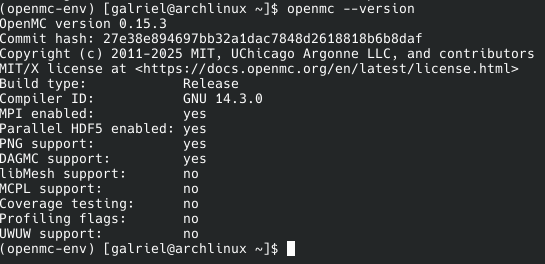
\includegraphics[width=0.8\linewidth]{Figures/FigureI-OpenMCversion.png}
    \label{fig-label-name}
    \caption{Screenshot of Terminal Depicting OpenMC Version}
\end{figure}
\\

\begin{figure}[h!]
    \centering
    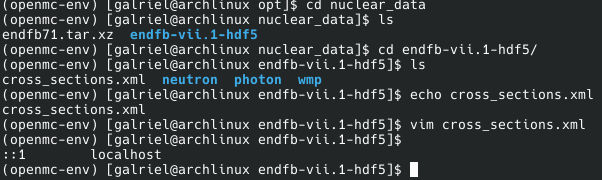
\includegraphics[width=0.8\linewidth]{Figures/FigureII-ENDF7.png}
    \label{fig-label-name}
    \caption{Screenshot of ENDF/B-VII.1 Folder}
\end{figure}

\section{Compute the Critical Enrichment of Uranium}
Create an infinite-homogeneous composition of pure uranium (metal). Then, use the
enrichment argument to specify the uranium enrichment. For example,
uranium.add$\_$element("U", 1.0, enrichment=4.0)
would specify a material with 4 $\%$ enriched (by mass) uranium.

As described in the slab.py example, an infinite-homogeneous composistion of pure uranium metal can be represented in an infinite slab (in the y-direction) with a width of 6.5 cm. Below is the written code to express what is written in the prompt. Be aware that I have setup my location for the cross_sections.xml file differently than what is provided in the example and lecture.

import openmc
# Point OpenMC to the cross_sections.xml file with all cross section data.
openmc.config["cross_sections"] = "/opt/nuclear_data/endfb-vii.1-hdf5/cross_sections.xml"
################################################################################
# Describe the materials of the problem.
################################################################################

uranium = openmc.Material()
uranium.add_element("U", 1.0, enrichment=4.0)
materials = openmc.Materials([uranium])
materials.export_to_xml()
################################################################################
# Describe the geometry of the problem.
################################################################################

width = 6.5

# Begin by defining a surface at the left and right.
left = openmc.XPlane(0.0)
left.boundary_type = "vacuum"
right = openmc.XPlane(width)
right.boundary_type = "vacuum"

# Combine surfaces together into a cell
cell = openmc.Cell()
cell.region = +left & -right
cell.fill = uranium

geom = openmc.Geometry([cell])
geom.export_to_xml()

################################################################################
# Configure the settings.
################################################################################

settings = openmc.Settings()
settings.particles = 100_000
settings.batches = 100 + 50
settings.inactive = 50
# Create an initial uniform spatial source distribution over the domain.
bounds = [0.0, 0.0, 0.0, width, 0.0, 0.0]
uniform_dist = openmc.stats.Box(bounds[:3], bounds[3:])
settings.source = openmc.IndependentSource(space=uniform_dist)
settings.run_mode = "eigenvalue"
settings.export_to_xml()
# Run in parallel with four threads.
openmc.run(threads=4)





\begin{itemize}

\item Perform a criticality search to find the enrichment of uranium metal that would be critical
in an infinite-homogeneous mixture.
\\

\item Without performing any additional calculations, using only your answer to 2(a), what
would be the critical radius of a sphere of 3.2 $\%$ enriched uranium? Explain your
reasoning
\end{itemize}

\subsection{Calculate the critical dimensions of High-Assay Low-Enriched Uranium (HALEU)}
Low-Enriched Uranium (LEU) is defined by the International Atomic Energy Agency (IAEA)
as < 20 $\%$ enriched uranium. Historically in the United States, enrichment has been limited
to < 5 $\%$ as an administrative control. Recent interest in advanced reactors, especially
fast-spectrum reactors like Sodium-cooled Fast Reactors (SFRs), has turned to HALEU to
achieve the uranium density requirements for these reactors. Generally speaking, HALEU is
defined as enrichments between 5 $\%$ and 20 $\%$.

You will compute the critical dimensions of HALEU for certain geometries.

\begin{itemize}
\item Compute the critical radius for a sphere of 20$\%$ enriched uranium.
\item Compute the critical radius for a one-dimensional cylinder (infinite in the z-direction) of 20 $\%$ enriched uranium.
\item Compute the critical width of a one-dimensional slab of 20$\%$ enriched uranium.
\item Consider you answer to Problem 2 (above). How would a facility that is currently
designed to handle 5 $\%$ enriched uranium need to be modified to accept 20 $\%$ enriched
uranium? Recall that criticality safety is always a balancing act. What are the competing
forces in this proposed design change
\end{itemize}

\newpage







%%%%% header and footer
\pagestyle{fancyplain}
\fancyhf{} %clear header and footer 
\renewcommand{\headrulewidth}{0pt} %set line thickness in header; uncomment as is to remove line
\rfoot{\fancyplain{}{\thepage}}
\nolinenumbers
%%%%%


%%%%%%% citations
%
%%% make sure $BIBREF contains the path to each bib file in .bashrc
%%% make sure Overleaf has the latexmkrc pointing to where the bib and bst are located
%
\bibliographystyle{nsf}
\setlength{\bibhang}{0pt}
\bibliography{references}
%
%%%%%%%







%\begin{figure}[h!]
%    \centering
%    \includegraphics[width=0.X\textwidth]{filename}
%    \caption{Descriptive caption}
%    \label{fig-label-name}
%\end{figure}




%%%%% formatting
    \renewcommand{\thesection}{\Roman{section}}
%%%%%


%    \section{\acs{mcp} input decks} \label{app-mcnp}



\end{appendices}


\end{document}
